\documentclass{article}

\usepackage{graphicx}
\usepackage{amsmath}
\usepackage{hyperref}
\usepackage{float}




\title{Meetrapport: Bepaling van de specifieke lading van een elektron}
\author{Koen Kruijt, Hanne Klapwijk}
\date{October 15, 2024}


\begin{document}
\maketitle

Klas: NH2.c \newline
Docent: Triemstra, T.

\newpage
\tableofcontents
\newpage
\section{Doel}
Het doel van de proef is om de specifieke lading van een elektron te bepalen. Dit wordt gedaan door een elektronenbundel in een magnetischveld af te schieten, de elektronen buigen dan af omdat ze geladen zijn. Door de diameter van de bundel en de sterkte van het magnetischveld te meten kan de specifieke lading worden bepaald.
Hier uit volgt ook de onderzoeksvraag: Wat is de specifieke lading van een elektron?

\section{Verwachtingen}
De verwachting is dat de waarde van de specifieke lading die gemeten wordt in de buurt komt van de theoretische waarde ($1.76 \times 10^{11} \frac{C}{kg}$\cite{masscharge}). De gebruikte apparatuur is een "PHYWE: Narrow-beam tube, Pair of Helmholtz coils".

Voor het uitrekenen van de waardes worden de volgende formules gebruikt:
\begin{equation}
	\frac{e}{m} = \frac{2U}{B^2r^2}
	\label{eq:specifiekelading}
\end{equation}
\begin{equation}
	B = 0,715\mu_0 \frac{n \cdot I}{R}
	\label{eq:magnetischveld}
\end{equation}

Waar $\frac{e}{m}$ de specifieke lading is, $U [v]$ de spanning op het elektronenkanon, $B [T]$ de magnetische veldsterkte, $r [m]$ de straal van de elektronenbundel, $\mu_0 [N\cdot A^{-2}]$ de magnetische permeabiliteit, $n [1]$ het aantal windingen van de spoel, $I [A]$ de stroomsterkte door de spoel en $R [m]$ de straal van de spoelen.

Uit \ref{eq:specifiekelading} volgt de volgende linearisatie:
\begin{equation}
	U =\frac{e}{m} \cdot B^2 \cdot r^2 \cdot \frac{1}{2}
	\label{eq:linearisatie}
\end{equation}
Die gebruikt kan worden om de specifieke lading te bepalen door middel het aflezen van de richtingscoëfficiënt.

\section{Schematische weergave van de opstelling}

\section{Resultaten}

%plot.png
\begin{figure}[h]
	\centering
	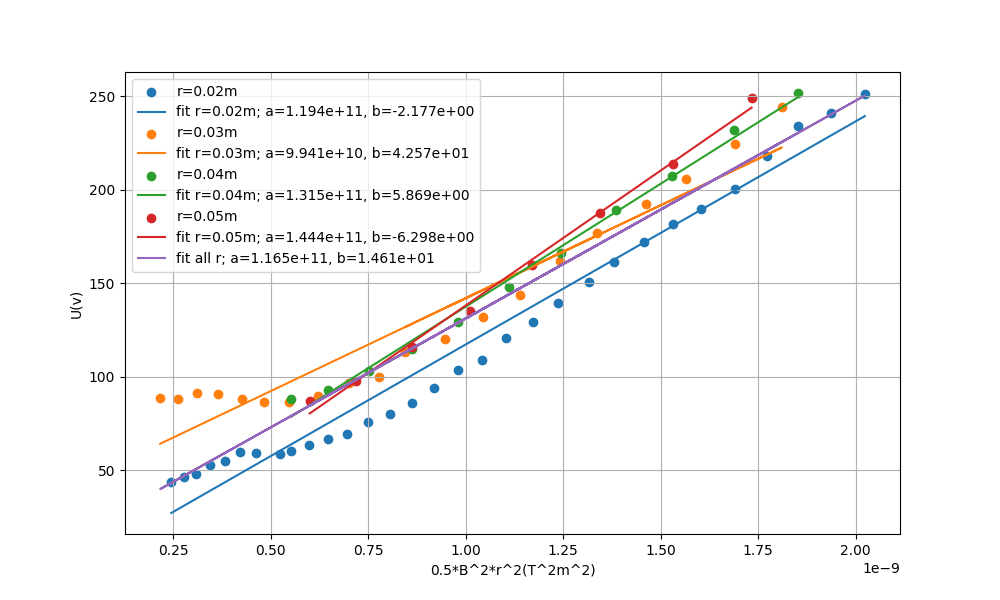
\includegraphics[width=0.7\textwidth]{plot.png}
	\caption{De gemeten waardes van de spanning en de magnetische veldsterkte}
	\label{fig:plot}

\section{Uitwerking \& discussie}

\section{Conclusie}




\end{document}